%En un máximo de 3 páginas formule en forma general su proyecto, donde usted se debe referir a
%los siguientes puntos:

\subsection{Definición del Problema}
	%Defina el contexto y el problema que pretende abordar en el marco de este proyecto. Incluya una
	%discusión bibliográfica que fundamente adecuadamente desde el punto de vista técnico su
	%proyecto.
	Siempre que existe una relación de cualquier tipo entre dos o más entidades,
	está la posibilidad que el \emph{medio} utilizado para la comunicación,
	sea perturbado por cualquier actividad fuera de dicho universo de conversación,
	como lo muestra la figura ~\ref{fig:fig1}.

	\begin{figure}[htp]
		\centering
		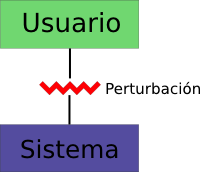
\includegraphics[scale=0.3]{img/user-sist}
		\caption{Comunicación Usuario-Sistema y sus perturbaciones}
		\label{fig:fig1}
	\end{figure}

	En el área de la informática, el manejo de información es un tema latente
	en todo sentido, por lo tanto para poder mantener la credibilidad y veracidad de
	dicha información, es necesario poder asegurar el medio de intercambio de datos,
	es aquí donde aparece el término de \emph{Control de Acceso Lógico},
	enfocado a sistemas y aplicaciones, siendo así la primera barrera a cualquier
	\emph{perturbación} que nuestro ambiente de transferencia de información pueda
	ser afectado.

	Para poder reducir la probabilidad de que las \emph{perturbaciones} tengan éxito,
	y puedan interferir la transferencia de información, se utilizan distintos métodos
	seguridad, ya sea mediante hardware, software o ambos, todos con el mismo fin de
	impedir un acceso inseguro.

	Es por lo dicho anteriormente que los \emph{Controles de Acceso lógico} son de vital
	importancia, pues permiten proteger los recursos en una amplia variedad de sistemas.
	Debido a la problemática señalada anteriormente, han llegado a surgir distintos tipos
	de sistemas para poder hacer interactuar herramientas y así establecer un cierto control
	en nuestro canal de comunicación, como es el caso del servicio del \emph{Java
	Authentication and Authorization Service}~\cite{paper1} que nos permite tener acceso a
	servicios de control de autenticación y acceso para distintas aplicaciones Java,
	sin dejar de lado algunos otros tipos de utilización,
	como lo es el caso de poder ayudar a remover ambigüedades de ciertas definiciones informales
	en un modelo de control, basado en una aplicación Java, convirtiéndola en una especie
	de máquina abstracta que se comporta bajo un conjunto de reglas~\cite{paper2}.

	Finalmente, cabe señalar que nuestra problemática aumenta notablemente cuando los recursos de
	nuestro sistema almacenan datos extremadamente sensibles, como ``información confidencial'',
	``documentos clasificados'', etc, por ésto es que claramente para solucionar nuestra situación
	necesitamos un sistema robusto, estableciendo alguna suerte de credenciales virtuales,
	para realizar ciertas autenticaciones, conteniendo así la información necesaria para poder
	autenticar a un sujeto frente a un servicio determinado~\cite{paper3}.
	

\subsection{Objetivos del Proyecto}
	%Defina el objetivo general del proyecto y los objetivos específicos que han identificado (detalle de
	%lo que quieren alcanzar), limitando adecuadamente el alcance del proyecto (qué cosas
	%definitivamente no abordarán).
	El objetivo principal de nuestro proyecto es:

\begin{itemize}
\item Implementar el modelo API de autenticación JAAS (Java Authentication and Authorization Service) para controlar el acceso, vía autenticación, a máquinas JBoss, a cargo del grupo 5. 
\end{itemize}
	Nuestros objetivos específicos son:

\begin{itemize}
\item Poder comunicarse con un Servidor de Directorios, como LDAP, o utilizar una base de datos para almacenar la información de los usuarios.
\item Utilizar JAAS, para autentificar vía  web a los usuarios que quieran ingresar a la máquina JBoss.
\item Dar acceso diferenciado a los usuarios, ya sean administrador o usuarios, para poder utilizar la maquina JBoss.
\end{itemize}

	Si bien abordaremos las bases de la autenticación, hay algunos puntos los cuales, por disponibilidad de tiempo, no podemos comprometernos a realizar, correspondiendo a las herramientas mas avanzadas de JAAS como:

\begin{itemize}
\item Autenticaciones múltiples bajo un solo dominio.
\item No utilizaremos JPam para la autenticación.
\end{itemize}

	
\subsection{Resultados Esperados}
	%Refiérase brevemente a los resultados que espera lograr con este trabajo y relaciónelos con los
	%entregables que debe contener el informe final; especialmente con el reporte técnico, material
	%complementario y demostración.
	Para nuestro proyecto pretendemos lograr implementar un sistema de autenticación JAAS, de manera
óptima para poder realizar las tareas de comunicación con un Sistema de Directorios, como LDAP, y
permitir la autenticación diferenciada en el ingreso a la máquina JBoss que implementarán nuestros
compañeros del grupo correspondiente. Esperamos comprender el sistema a fondo, utilizando las correctas
directrices de seguridad que éste posee y dar un servicio óptimo de autenticación de usuarios para los
demás grupos que utilicen el sistema.
	
También, y a pesar de no estar en nuestros objetivos específicos, podríamos probar la implementación de
JAAS en otros servicios de autenticación como Pam, a través del puente que proporciona JPam y comparar
las ventajas y desventajas que estos dos sistemas poseen y ver como a su vez se puedan ver
complementados.
		


